\documentclass[]{subook}
% \usepackage{showframe}
\usepackage{graphicx}
\usepackage{subcaption}

\begin{document}
\pagestyle{empty}
\newgeometry{paper=a4paper,marginparwidth=0pt,marginparsep=0pt,hoffset=0in,voffset=0in}
\setcounter{page}{0}
% % temporary titles
% command to provide stretchy vertical space in proportion



\begin{center}
\bfseries
\nbvspace[1]
\Huge
{\nbtitlestretch\huge
Subook}

\nbvspace[1]
\normalsize

TO WHICH IS ADDED MANY USEFUL ONE\\
LINERS AND CODE SO THAT\\
YOU CAN AWK LIKE A HAWK
\nbvspace[1]
\small BY\\
\Large Changxing Su\\[0.5em]
\footnotesize An Human 

\nbvspace[2]

% \includegraphics[width=1.5in]{./graphics/pic37}
\nbvspace[3]
\normalsize

DOHA\\
\large
PUBLISHED IN THE WILD
\nbvspace[1]
\end{center}
% \maketitle

% \pagestyle{empty} % Disable headers and footers for the following pages
\dominitoc% Initialization


\tableofcontents % Print the table of contents itself


%% //FIXME:The page style of contents
\restoregeometry

\pagestyle{fancy} % Enable headers and footers again
\part{User Manual}

\chapter{Introduction}
\minitoc
% \printMarginPartialToc
As the year went on, I started typesetting my personal notes during class and realized that the \LaTeX  format, 
while great for publications and lecture notes in general, was lacking a few small but useful template for me.

\section{Required Packages}\label{sec:reqpackages}
For \textit{Subook,} the following packages are required
\begin{center}
    \texttt{marginnote, sidenotes, fancyhdr, titlesec, geometry, and tcolorbox.}
\end{center}
For a brief summary, the \texttt{marginnote}, \texttt{sidenote}, \texttt{titlesec}, 
and \texttt{tcolorbox} packages are used in creating the \texttt{$\backslash$part} environment, 
the package \texttt{geometry} is used globally to set the page width, page height, 
and margin width, and finally, \texttt{fancyhdr}, 
which is overridden on the title page, 
the contents page, and the \texttt{$\backslash$part} page, sets the header for the body.


\section{License}\label{sec:license}
This work may be distributed and/or modified under the conditions of the LaTeX Project Public License, 
either version 1.3 of this license or (at your option) any later version. 
The latest version of this license is found in  \url{http://www.latex-project.org/lppl.txt}, 
and version 1.3 or later is part of all distributions of LaTeX version 2005/12/01 or later. 
The current maintainer of this work is Changxing Su.

\section{Features}\label{sec:Features}

\textit{Subook} includes the following:
	\begin{enumerate}
		\item Several mathematics and physics packages.
		\item Margins and margin environments for tables, figures, and asides.
		\item \TeX\ shortcuts for various math scripts namely vector bold math, \texttt{mathbb}, \texttt{mathfrak}, and \texttt{mathcal}.
		\item \texttt{amsthm} integrations and special environments for theorems, lemmas, proofs, definitions, examples, and remarks.\
		\item Stylized support for the \texttt{part} environment.
		\item A fullpage environment that spans across the text width and the margin for longer equations and horizontal figures.
	\end{enumerate}
    Each of these will be discussed in the following subsections.


\section{\TeX\ Shortcuts}\label{sec:shortcuts}
\textit{subook} comes built in with a minimal set of keyboard shortcuts for a few special characters. All of these shortcuts can be found in \texttt{subook.cls} just under
\begin{verbatim}
% ----------------------------------------------------------------------
%           User Created Commands
% ----------------------------------------------------------------------
...
\end{verbatim}
If one has their own macros\marginpar[right]{Most people have their own shortcuts for commonly used mathematics, such as derivatives or integrals. For those looking for physics shortcuts, the {excellent} \texttt{physics} package (automatically included in \textit{subook}) has possible everything that one can imagine.} then simply add it under this area. 


\section{\texttt{amsthm} Environments}\label{Sub:Special}
\texttt{amsthm} environments are defined as usual being enclosed by \texttt{$\backslash$begin\{environment\}}$\cdots$ \texttt{$\backslash$end\{environment\}} 
and most have been modified ostensibly from the original \texttt{amsthm} presets. 
Primarily, most environments, 
with the exception of the exercise environment, are now integrated with the wonderful \texttt{tcolorbox} package. 
Note that the counting for \texttt{theorems} and \texttt{lemmas} is distinct from the counting for \texttt{definitions}. 
Also note that the \texttt{breakable} for \texttt{tcolorbox} allows these environments to span multiple pages.
All of these environment and the associated \texttt{tcolorbox} are provided by the  code in \texttt{subook.cls} just under \lecture.
\begin{verbatim}
    % ----------------------------------------------------------------------
    %                         User Created Environments 
    % ----------------------------------------------------------------------
    ...
    %% ------------------------------ tcolorbox  ---------------------------
    ...
\end{verbatim}

\begin{definition}[Test]
    The \texttt{definition} environment
\end{definition}


\begin{lemma}[Test]
    The \texttt{lemma} environment
\end{lemma}

\begin{theorem}[Test]
    The \texttt{theorem} environment
\end{theorem}

\begin{corollary}[Test]
    The \texttt{corollary} environment
\end{corollary}

\begin{proposition}[Test]
    The \texttt{proposition} environment
\end{proposition}


\begin{example}[Test]
    The \texttt{example} environment
\end{example}

\begin{proof}
    The \texttt{proof} environment
\end{proof}


\begin{remark}
    The \texttt{remark} environment
\end{remark}

\begin{assumption}
asdasd
\end{assumption}

\begin{exercise}
sdadsa
\end{exercise}
\begin{tbox}{Some extra box environment}
    The \texttt{something extra} environment
\end{tbox}

% \begin{examplebox}{Test}
%     I use my ``examplebox'' as usual text and margin figure work as they should be but I want my example box spread out to the right margin on an odd page, breakable, and spread out to the left margin on the even page.
%     \tcblower
%     I use my ``examplebox'' as usual text and margin figure work as they should be but I want my example box spread out to the right margin on an odd page, breakable, and spread out to the left margin on the even page.
% \end{examplebox}

\subsection{\texttt{tcolorbox} Environment and Known Issues}
\label{ssub:tcolorbox environments_and_known_issues}


The \texttt{breakable} should allow the \texttt{proof} environment to span multiple pages. If one wishes to change the color, simply modify the line which states \texttt{borderline west=\{1pt\}} \texttt{\{0pt\}\{blue\}}. The first numeric value dictates the width of the line, the second dictates how close it is away from the \textit{left} margin, while the last argument obviously dictates the color. This code could also be used to change any of the other \texttt{amsthm} environments
\marginpar{
    \centering
    \includegraphics[width=0.4\textwidth]{example-image-a}
    \captionof{figure}{marginfigure}}.


\section{Fullpage Environment}\label{Sec: Fullpage}

\begin{fullpage}
    The \texttt{fullpage} environment is defined by
    \begin{center}
        \texttt{$\backslash$begin\{fullpage\}}\\
        $\cdots$\\
        \texttt{$\backslash$end\{fullpage\}}
    \end{center}
    with the width of the \texttt{fullpage} environment given by \texttt{$\backslash$textwidth}+\texttt{$\backslash$marginparsep}+\texttt{$\backslash$marginparwidth}
    There are some clear benefits of having use of the full page at times. Suppose that one wants to place a figure that cannot fit into the margins, or if an equation is quite long and it bleeds into
     the margin, 
    then the \texttt{fullpage} environment can both clearly separate these from the surrounding text and allot for the dimensions without hassle. 
%% //FIXME  : When using figure enviorment, recipe terminated with error by message"Float(s) lost." 
    % \begin{figure}

    \centering
        \includegraphics{img/f08Young.pdf}
        \captionof{figure}{Figure caption}
        \label{fig:example} % Unique label used for referencing the figure in-text
    %     %\addcontentsline{toc}{figure}{Figure \ref{fig:placeholder}} % Uncomment to add the figure to the table of contents
    % \end{figure}
    \begin{definition}[big box]
        dsdd
    \end{definition}
\end{fullpage}

\texttt{Figure} is a floating environment and \texttt{minipage} is, unfortunately, not. Therefore, if you put a floating object inside a non-floating minipage, you will get an error.One way is to avoid using figure entirely. This can be done with help of the caption package (with its captionof facility, so that you can have a caption for the figure):
%% solution from https://tex.stackexchange.com/questions/55337/how-to-use-figure-inside-a-minipage
\begin{lstlisting}
    \centering
        \includegraphics{img/f08Young.pdf}
        \captionof{figure}{Figure caption}
        \label{fig:example} % Unique label used for referencing the figure 
\end{lstlisting}
Table\marginpar{\centering
\begin{tabular}{lll}
\toprule
1 & 1 & 1\\
\midrule
1 & 1 & 0.562 \\
2 & 1 & 0.910 \\
3 & 11 & 0.296 \\
\bottomrule
\end{tabular}
\captionof{table}{Sophisticated margin table}
}The genomes of chimpanzees and humans are 99.9\% identical, yet the differences between the two species are vast. The relatively few differences in genetic endowment must explain \marginpar[right]{dsdsdsdsd}the possession of language by humans, the extraordinary athleticism of chimpanzees, and myriad other differences. Genomic comparison is allowing researchers to identify candidate genes linked to divergences in the developmental programs of humans and the other primates

\lipsum[2-4]
Tikz\marginpar{		\begin{center}
    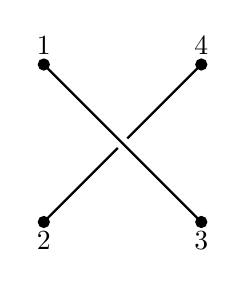
\begin{tikzpicture}
        \draw[black,thick] (-1,-1) -- (-.06,-.06);
        \draw[black,thick] (.06,.06) -- (1,1);
        \draw[black,thick] (-1,1) -- (1,-1);
        \filldraw[black] (-1,-1) circle (2pt) node[anchor=north] {2};
        \filldraw[black] (-1,1) circle (2pt) node[anchor=south] {1};
        \filldraw[black] (1,-1) circle (2pt) node[anchor=north] {3};
        \filldraw[black] (1,1) circle (2pt) node[anchor=south] {4};
    \end{tikzpicture}
\end{center}
\captionof{figure}{Marginfigure: Tikz}}


\lipsum[2-4]\marginpar{\begin{theorem}[Test asdsadsads]
    The \texttt{theorem} environment
\end{theorem}}
\newpage
\chapter{Test ss}
 
    \epigraph{``Begin at the beginning," the King said gravely, ``and go on till you come to the end: then stop."}{--- \textup{Lewis Carroll}, Alice in Wonderland}
%     \minitoc
%     \section{test}

    The genomes of chimpanzees and humans are 99.9\% identical, yet the differences between the two species are vast. The relatively few differences in genetic endowment must explain \marginpar[right]{dsdsdsdsd}the possession of language by humans, the extraordinary athleticism of chimpanzees, and myriad other differences. Genomic comparison is allowing researchers to identify candidate genes linked to divergences in the developmental programs of humans and the other primates
%     % \marginnote{%
%     % \centering
%     % \begin{tabular}{lll}
%     % \toprule
%     % 1 & 1 & 1\\
%     % \midrule
%     % 1 & 1 & 0.562 \\
%     % 2 & 1 & 0.910 \\
%     % 3 & 11 & 0.296 \\
%     % \bottomrule
%     % \end{tabular}
%     % \captionof{table}{Sophisticated margin table}
%     % } 
%     and to the emergence of complex functions such as language. The picture will become clearer only as more primate genomes become available for comparison with the human genome.



    \section{sdadsad}
    sdasadsadadsdsadsasd sdaasd
    \lipsum[1-3]
    \subsection{dsadsad}
    dsadasds
    \lipsum[1-4]
    \section{dsad}
    \lipsum[2-6]

%     % \begin{figure}[b]
%     %     \inneralign{\includegraphics{f08Young}}
%     %     \caption{A point source produces coherent
%     %     (locked phases) light.  When this light which traverses two
%     %    slits and arrives at a screen it produces a fringe pattern.
%     %     }
%     % \end{figure}
    
% \begin{definition}[ds]
%     \begin{equation}
%         \begin{aligned}
%             \mathcal{L} _{\rm{BCE}}(\boldsymbol{\hat{y} },\boldsymbol{y})&=\sum ^N_{i=1}-y^{(i)}\log (\hat{y}^{(i)})- (1-y^{(i)})\log (1-\hat{y}^{(i)})\\
%             &=\sum^N_{i=1}
%             \begin{cases}
%             -\log (\hat{y}^{(i)}),  & \text{for $y^{(i)}=1$} \\
%             -\log (1-\hat{y}^{(i)}), & \text{for $y^{(i)}=0$}
%             \end{cases}
%         \end{aligned}
%     \end{equation}
% \end{definition}


% \lipsum[2]
% \begin{theorem}[ad]
%     abs
% \end{theorem}

% assured
% \begin{lemma}[asd]
%     sdsd
% \end{lemma}


% \lipsum[1]
% \begin{postulate}
%     dsadsa
% \end{postulate}
% \lipsum[4]
% \begin{proof}
%     dsad
% \end{proof}
% \lipsum[4-6]

% % \begin{remark}
% %     borderline west
% % \end{remark}

% \begin{examplebox}{}
%     I use my ``examplebox'' as usual text and margin figure work as they should be but I want my example box spread out to the right margin on an odd page, breakable, and spread out to the left margin on the even page.
%     \tcblower
%     I use my ``examplebox'' as usual text and margin figure work as they should be but I want my example box spread out to the right margin on an odd page, breakable, and spread out to the left margin on the even page.
%   \end{examplebox}

% \lipsum[2-5]
% \begin{corollary}
%     sadsd
% \end{corollary}
% \lipsum[3]
% \begin{proposition}[dsaf]
%     dsadasd
% \end{proposition}

% \begin{tbox}{some extra box}
%     dsadasd
%     Similarly, the differences in genetic endowment among humans are vanishingly small compared with the differences between humans and chimpanzees, yet these differences account for human\citep{li2022limb} variety—including differences in health and in susceptibility to chronic diseases. We have much to learn about the variability in genomic sequence among humans, and the availability of genomic information will almost certainly transform medical diagnosis and treatment. Several monumental studies in which the entire
% \end{tbox}


% A listings example:
% \begin{lstlisting}[language=Python, caption=Python example]
%     import numpy as np

%     def incmatrix(genl1,genl2):
%         m = len(genl1)
%         n = len(genl2)
%         M = None #to become the incidence matrix
%         VT = np.zeros((n*m,1), int)  #dummy variable
        
%         #compute the bitwise xor matrix
%         M1 = bitxormatrix(genl1)
%         M2 = np.triu(bitxormatrix(genl2),1) 
    
%         for i in range(m-1):
%             for j in range(i+1, m):
%                 [r,c] = np.where(M2 == M1[i,j])
%                 for k in range(len(r)):
%                     VT[(i)*n + r[k]] = 1;
%                     VT[(i)*n + c[k]] = 1;
%                     VT[(j)*n + r[k]] = 1;
%                     VT[(j)*n + c[k]] = 1;
                    
%                     if M is None:
%                         M = np.copy(VT)
%                     else:
%                         M = np.concatenate((M, VT), 1)
                    
%                     VT = np.zeros((n*m,1), int)
        
%         return M
%     \end{lstlisting}
% \bibliography{reference}

\part{very big}


\chapter{ds dsd}
% \minitoc

\section{dsadsa}

\lipsum[1-6]
% and the availability of genomic information will almost certainly transform medical diagnosis and treatment. Several monumental studies in which the entire\citep{LevelUpTheGuidetoGreatVideoGameDesign_Rogers}.
\subsection{fff}
\lipsum[2]
\section{dasdsa}
\lipsum[2-4]
\bibliography{reference}
\part{three}
\chapter{[asdaf]}
\section{das}
\lipsum[1-3]

\section{ffsad}
\lipsum[1-6]


\part{probability}

\chapter{Pro}
\newcommand{\cX}{\mathcal{X}}
\newcommand{\cY}{\mathcal{Y}}

\section{Review and Overview}
In this lecture we delineate a mathematical framework for supervised learning. We focus on regression problems and define the notion of the loss/risk associated with a model. We then analyze a particular loss function (the squared loss) in a general setting, then specialize our result to the case of linear models. We next define the notion of parameterized families of hypotheses and the maximum likelihood estimate, and we conclude with an asymptotic result relating the training MLE to the true maximum likelihood parameter.

\section{Formulation of supervised learning}
We begin by constructing a mathematical framework for prediction problems. Our framework consists of the following elements:
\begin{enumerate}
	\item A space of possible data points $\cX$.
	\item A space of possible labels $\cY$.
	\item A joint probability distribution $P$ on $\cX\times \cY$. We assume that our training data consists of $n$ points $$(x^{(1)}, y^{(1)}), \: \ldots, \: (x^{(n)}, y^{(n)}) \: \iid \: P$$ each drawn independently from $P$.
	\item A prediction function/model $f: \cX\rightarrow \cY$.
	\item A loss function $\ell: \cY\times \cY\rightarrow \mathbb{R}$. We will usually assume that $\ell$ is bounded below by some constant, typically $0$.
\end{enumerate}
Given the prediction function $f$ and the loss function $\ell$, the loss of an example is $\ell(f(x),y)$. We can then define the \textit{expected risk} (or \textit{expected loss}, or \textit{population risk})
$$L(f) \defn \E_{(x,y)\sim P} [\ell(f(x),y)].$$ Our goal will be to obtain a small expected loss. Often it will be infeasible to consider all possible models $f$, so we may restrict ourselves to a certain family of hypotheses $\mathcal{F}$. In this case, we define the \textit{excess risk} of a model $f$ as $$L(f) - \inf_{g\in\mathcal{F}} L(g).$$ This gives us a measure of how well our model fits the data relative to the best we can hope to do within our set of options $\mathcal{F}$.

Within this framework, there are two main types of problems we will consider: \textit{regression} problems, where the set of labels is $\cY=\mathbb{R}$; and \textit{classification} problems, where the set of labels is some finite set $\cY=\{1,\ldots,k\}$. We will focus on regression problems in this lecture.

\section{Regression problems and squared loss}
We consider the regression problem of predicting $y$ given $x$. We take as our loss function the \textit{squared loss} $$\ell(\hat{y},y) = (\hat{y}-y)^2, \hspace{.5in} L(f) = \E_{(x,y)\sim P}[(f(x)-y)^2].$$ In this setting, we can decompose the risk in a very informative way.
\begin{lemma}[Decomposition of loss] \label{decomp}
Under the squared loss, we have the decomposition $$L(f) = \E_{x\sim P_x} [(f(x)-\E[y \: | \: x])^2] + \E_{x\sim P_x}[\Var(y\: | \:x)]$$ where $P_x$ is the marginal distribution of $x$.
\end{lemma}
The second term in this expansion is the intrisic variable of the label; it gives a lower bound on the loss we can achieve. Since the first term in the decomposition is nonnegative, it is an immediate corrolary that the optimal model is $f(x) = \E[y \: | \: x]$.

In order to prove Lemma 1, we make use of the following claim.
\begin{center}
    If $Z$ is a random variable and $a$ is a constant, then $$\E[(Z-a)^2] = (\E[Z]-a)^2 + \Var(Z).$$
\end{center}


The proof of this claim is left as an exercise on HW 0. We are now ready to prove Lemma 1.
\begin{proof}[Proof of Lemma \ref{decomp}]
We have
\begin{align*}
    L(f) &= \E[(f(x)-y)^2] \\
    &= \E_{x\sim P_x}[\E_{P_{y \; | \;x}}[(f(x)-y)^2\: | \: x]] & \mathrm{(Law~{} of~{} total~{} expectation)} \\
    &= \E_{x\sim P_x}[(f(x)-\E[y \: | \: x])^2 + \Var(y \: | \: x)]. & \mathrm{(Claim~{} \ref{claim:variance})}
\end{align*}
Note that Claim \ref{claim:variance} holds in the third equation since $f(x)$ is a constant when we have conditioned on $x$. The desired result follows from linearity of expectation.
\end{proof}
Lemma \ref{decomp} gives us a general lower bound on risk under squared loss. If we impose more structure on the set of hypotheses $\mathcal{F}$ from which we can select $f$, we can gain more information on the risk.

\section{Linear regression under squared loss}
A commonly used choice of hypotheses is the set of linear functions: $$\mathcal{F} = \{f: \mathbb{R}^d \rightarrow \mathbb{R} \: | \: f(x) = w^\top x, \: w\in \mathbb{R}^d\}.$$ For $f\in\mathcal{F}$, we then have $$L(f) = L(w) = \E[(w^\top x-y)^2].$$ Henceforth, we will denote $w^* \in \mathrm{argmin}_{w\in\mathbb{R}^d} L(w)$ and $\hat{w}$ will denote a model learned from training data.

One may ask why we have only allowed linear functions with $0$ instead of allowing a nonzero intercept. Actually, the framework we have outlined above is enough to accomodate nonzero intercepts. If we wish to analyze the function $w^\top x + b$, we can simply set $\tilde{x} = (x,1)$ and $\tilde{w} = (w,b)$. Then $\tilde{w}^\top \tilde{x} = w^\top x + b$ and we have reduced to the case of $0$ intercept.

When we restrict to linear models, we can further decompose the risk under squared loss.
\begin{lemma} \label{lin}
With $w^*\in \mathrm{argmin}_{w\in \mathbb{R}^d}L(w)$, we have \begin{equation}\label{decomp2}L(\hat{w}) = \E_x [\Var(y \: | \: x)] + \E_x[(\E[y\: | \: x]-w^{*\top} x)^2] + \E_x[(w^{*\top} x-\hat{w}^\top x)^2].\end{equation}
\end{lemma}
The second term in equation (\ref{decomp2}) can be thought of as the approximation error incurred by linear models. The third term can be interpreted as the estimation error we incur from having only a finite sample.
\begin{proof}
Define $g(\hat{w}) \defn \E[(\E[y\: | \: x]-\hat{w}^\top x)^2]$. By Lemma \ref{decomp}, \begin{equation}\label{lem1}L(\hat{w}) = \E[\Var(y\: | \: x)] + g(\hat{w}).\end{equation} Observe that since $w^*\in \mathrm{argmin} L(w)$, $\nabla L(w^*)=0$. Furthermore, since $\E_x[\Var(y\: | \: x)]$ is a constant with respect to $w$, we have
\begin{align*}
    \nabla L(w) &= \nabla g(w) \\
    &= \E[\nabla_w(\E(y\: | \: x) -w^\top x)^2] \\
    &= 2\E[(\E(y\: | \: x) - w^\top x)x].
\end{align*}
Since $\nabla L(w^*)=0$ we have \begin{equation}\label{vanish}\E[(\E[y \: | \: x]-w^{*\top}x)x]=0.\end{equation} Next, we expand:
\begin{align*}
    g(\hat{w}) &= \E[(\E[y\: | \: x]-\hat{w}^\top x)^2] \\
    &= \E[((\E[y\: | \:x]-w^{*\top}x)-(\hat{w}^\top x-w^{*\top}x))^2] \\
    &=\E[(\E[y\: | \: x] - w^{*\top}x)^2 + (\hat{w}^\top x - w^{*\top}x)^2] \\
    &\hspace{.25in} -2\E[(\E[y \: | \: x] - w^{*\top}x)(\hat{w}^\top x-w^{*\top}x)].
\end{align*}
Finally, observe that $$\E[(\E[y\: | \:x] - w^{*\top}x)(\hat{w}^\top x - w^{*\top}x)] = (\hat{w}^\top - w^{*\top})\E[(\E[y\:|\:x]-w^{*\top}x)x].$$ By equation (\ref{vanish}), this quantity vanishes and it follows that
\begin{equation}\label{g}g(\hat{w}) = \E[(\E[y\: | \: x] - w^{*\top}x)^2] + \E[(\hat{w}^\top x - w^{*\top}x)^2].\end{equation} Combining equations (\ref{lem1}) and (\ref{g}) gives the desired result. 
\end{proof}

\section{Parameterized families of hypotheses}
Linear models are one type of \textit{parameterized family} of hypotheses. In general, a parameterized family is given by a parameter space $\Theta$. For each $\theta\in\Theta$ there is a hypothesis $f_\theta(x)$, sometimes written $f(\theta; x)$. In this case we may write the loss function as $$\ell(f_\theta(x),y) = \ell((x,y),\theta).$$ In the special case of linear functions, our parameter space is $\Theta = \mathbb{R}^d$ and for $\theta \in \Theta$ we have $f_\theta(x) = \theta^\top x.$

\subsection{Well-specified case and maximum likelihood}
In the well-specified case, $P_\theta(y\: | \: x)$ is a family of distributions parameterized by $\theta\in\Theta$, and $y\: | \: x \sim P_{\theta^*}(y\: | \: x)$ is distributed according to some ground truth parameter $\theta^*$. We define the \textit{maximum likelihood} loss function by $$\ell((x,y),\theta) = -\log P_\theta(y\: | \: x),$$ so that minimizing the loss function is equivalent to maximizing the likelihood of the data.

For example, suppose that $y\: | \: x$ is Gaussian distributed with mean $\theta^{*\top}x$ and variance $1$, i.e. $y\: | \: x \sim N(\theta^{*\top}x, 1)$. The likelihood is then
\begin{align*}
    \ell((x,y),\theta) &= -\log P_\theta(y\: | \:x) \\
    &= -\log \exp\left(-\frac{(y-\theta^\top x)^2}{2}\right) + c \\
    &= \frac{(y-\theta^\top x)^2}{2} + c
\end{align*}
where $c$ is the log of the normalizing constant. This computation shows that in the Gaussian setting, minimizing the squared loss actually recovers the MLE.

\section{Training loss}
Often we do not know the true underlying distribution $P$ with which to compute the expected loss. In these cases we need to use an approximation based on the data we do have. This motivates our definition of the \textit{training loss} $$\hat{L}(\theta) \defn \frac1n \sum_{i=1}^n \ell((x^{(i)},y^{(i)}),\theta).$$ In the special case of maximum likelihood, we have $\hat{L}(\theta) = -\frac1n \sum_{i=1}^n \log p_\theta(y^{(i)}\: | \:x^{(i)})$. We define the \textit{maximum likelihood estimator} $$\hat{\theta}_{\mathrm{MLE}} \in \mathrm{argmin}_{\theta\in\Theta} \hat{L}(\theta).$$ This approximation is ``good" in the sense that as $n\rightarrow\infty$, the minimizer of the training loss $\hat{\theta}_\mathrm{MLE}$ approaches the true maximum likelihood parameter $\theta^*$. The following theorem quantifies this fact.
\begin{theorem}[Asymptotic of MLE] \label{mle}
  Assume $\nabla^2 L(\theta^*)$ is full rank. Let $\hat{\theta} = \hat{\theta}_{\mathrm{MLE}}$ and $$Q \defn \E_{(x,y)\sim P}[\nabla_\theta(\log p_\theta(y\: | \: x))(\theta^*) \nabla_\theta(\log p_\theta(y\: | \: x)(\theta^*)^\top].$$
  Assuming that $\hat{\theta}=\hat{\theta}_n\stackrel{\tiny p}{\rightarrow}\theta^\star$ (i.e. consistency) and under appropriate regularity conditions,  $$\sqrt{n}(\hat{\theta}-\theta^*)\stackrel{\tiny d}{\rightarrow} N(0, Q^{-1}) \textup{ and } n(L(\hat{\theta}) - L(\theta^*))\stackrel{\tiny d}{\rightarrow} \frac12 \chi^2(p).$$ as $n\rightarrow\infty$, where $p$ is the dimension of $\theta$ and $\chi^2(p)$ is the distribution of the sum of the squares of $p$ i.i.d. standard Gaussian random variables.
\end{theorem}

\begin{remark}
    The positive definiteness of the Hessian $\nabla^2 L(\theta^\ast)$ guarantees that identifiability holds \emph{locally} (in a neighborhood of $\theta^\ast$), but does not imply identifiability because of a lack of \emph{global} information. 

To give a counter-example, suppose $\theta^\ast$ is the global minimizer of $L$ and the Hessian is positive definite, but there exists a sequence of $\theta_n$ such that $\|\theta_n-\theta^\ast\|=n$ but $L(\theta_n)=L(\theta^\ast)+1/n$, then the identifiability is violated: the inf is not strictly greater than but equal to $L(\theta^\ast)$. The reason is that the Hessian does not reveal information about $L$ outside an infinitesimal neighborhood of $\theta^\ast$.

One way to exclude such adversarial case is to assume convexity: when $L$ is convex, a local strong growth implies global growth and thus identifiability
\end{remark}


\begin{example}[fasd]
    sdadasd
\end{example}

\end{document}